\documentclass[12pt]{article}

%\usepackage{fullpage}
%\usepackage[top=1in, bottom=1in, left=1in, left=1in, right=1in]{geometry}
\usepackage[margin=1in, paperwidth=8.5in, paperheight=11in]{geometry}
\usepackage{graphicx}
\usepackage{subcaption}
\usepackage{amsmath}
\usepackage{mathtools}

\newcommand{\argmin}{\operatornamewithlimits{argmin}}

\begin{document}

\title{UT Machine Learning: HomeWork1}
\author{Mohamad amin Katebsaber}
\date{\today}
\maketitle

\section{Class Summary}

Machine learning is a field of study in which we design proper instructions (algorithms) for computers, enabling them to learn for themselfs. Generally speaking based on the way computers improve using each algorithm, we can divide them into three types:

\begin{enumerate}
\item Supervised Learning 
\item Unsupervised Learning
\item Reinforcement Learning
\end{enumerate}

\subsection{Supervised Learning}
Supervised Learning algorithms can be considered as functions that map $input$ space to $output$ space. In this manner, $input$ space ($X$) is a set of examples, each of which consisting one or several features that the $output$ space ($Y$) depends upon. Here the objective is to best approximate the mapping function $(f)$ such that new datapoints ($x\in\mathcal{X}$) can be accurately mapped to $output$ space $Y$.Generaly there are two types of Supervised Learning based on the $output$ space:
\begin{enumerate}
\item Regression: If the $output$ space is numerical (continuous). i.e: Prdiction of Housing price in Tehran based on house area and number of rooms.
\item Classification: If the $output$ space is categorical (descrete). i.e: Identification of digits (Predicting a label between 0-9) based on pixel intensities.
\end{enumerate}

In Regression setting we aim to predict a real value on the calculated hyperplane but in Classification setting the calculated hyperplane is used as a boundary to devide input space to several zones (Figure \ref{fig:reg_clas}).
\begin{figure}[h!]
  \centering
  \begin{subfigure}[b]{0.4\linewidth}
    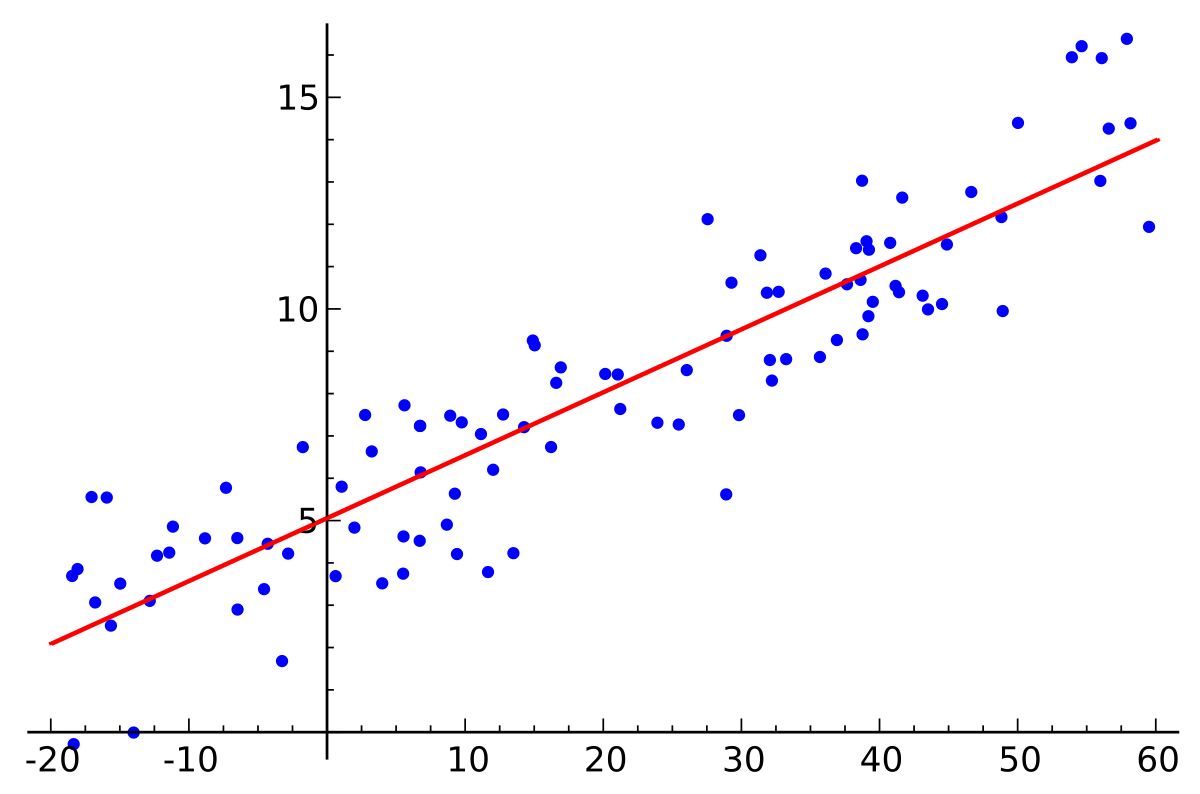
\includegraphics[width=\linewidth]{./images/regression.png}
    \caption{Regression}
  \end{subfigure} 
  \begin{subfigure}[b]{0.4\linewidth}
    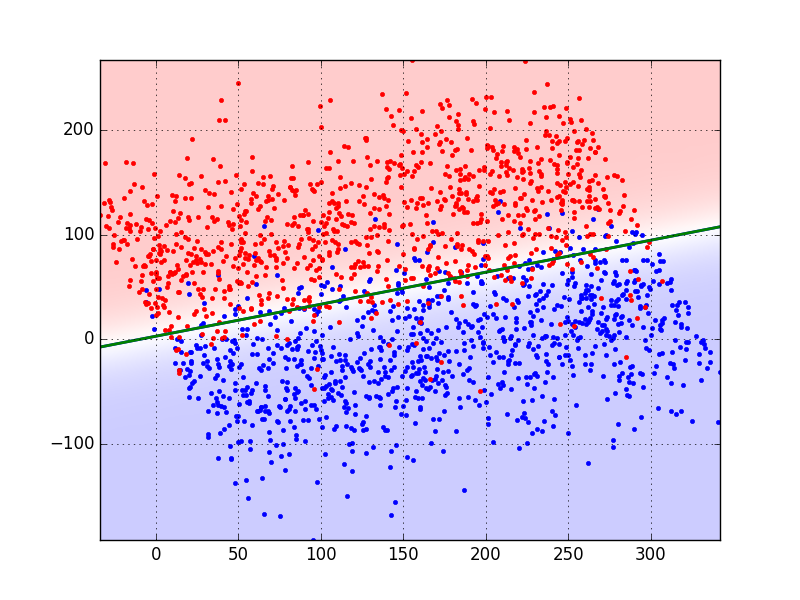
\includegraphics[width=\linewidth]{./images/classification.png}
    \caption{Classification}
  \end{subfigure}
  \caption{Regression vs Classification}
  \label{fig:reg_clas}
\end{figure}

\subsection{Unsupervised Learning}
Unsupervised Learning is referred to a class of algorithms capable of learning previously unknows patterns among $input data$ (there is no defined label for data points). These kind of algorithms are generally used for addressing two types of problem settings:
\begin{enumerate}
\item Clustering: In this setting we aim to group data space based upon features that represent the $input data$. Clustering is used when the $input$ space is discrete (Figure \ref{fig:tsne}-a).
\item Dimensionality reduction: In Machine Learning problems there are often too many features to be considered for defining the $input$ space. In many cases most of these features are by some means correlated and therefore redundant. Dimensionality reduction is the process of reducing the number of features decribing $input$ space based on afformentioned correlation, resulting in model's simplicity. This technique is often used when our $input$ space is continuous (Figure \ref{fig:tsne}-b).
\begin{figure}[h!]
  \centering  
  \begin{subfigure}[b]{0.4\linewidth}
  	\centering
    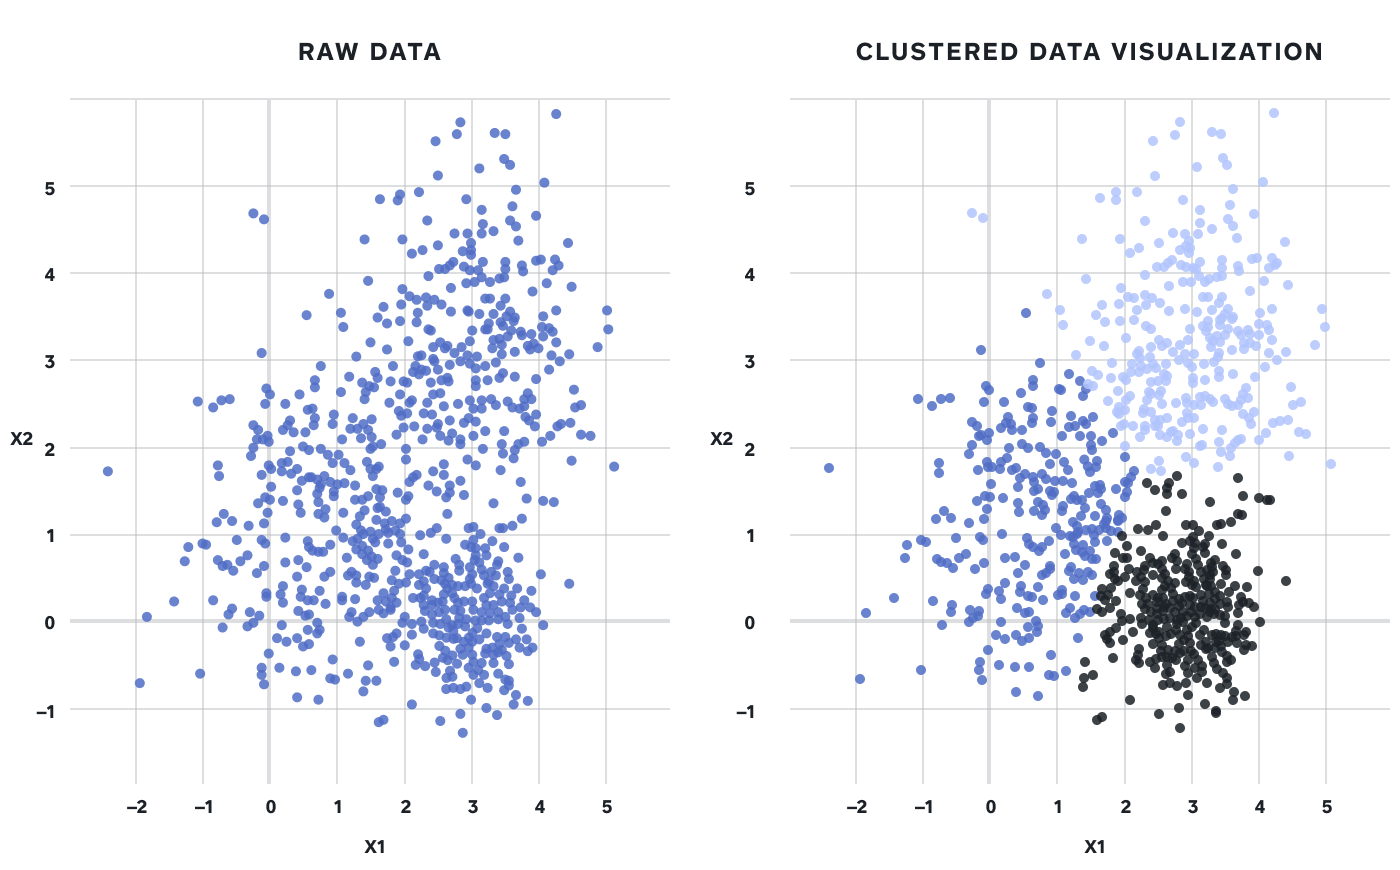
\includegraphics[width=\linewidth]{./images/clustering.png}
    \caption{Clustering}
  \end{subfigure} 
  \begin{subfigure}[b]{0.4\linewidth}
    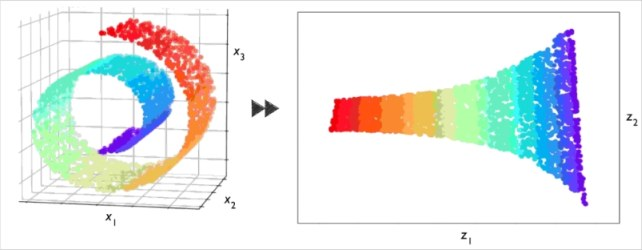
\includegraphics[width=\linewidth]{./images/reduction.jpg}
    \caption{Dimensionality reduction}
  \end{subfigure}
  \caption{Dimentionality Reduction}
  \label{fig:tsne}
\end{figure}
\end{enumerate}

As an example for Uunsupervised Learning we can name Blind Source Separation. Assume that you are in cocktail party where lots of individuals are talking together. In this house there are four microphones recording conversations from different points in the room. It can be concluded that depending on the position of each microphone and its proximity to a conversation, each microphone will record a specific signal. Problem of interest is about separation of signals related to each conversation from other signals (Figure \ref{fig:bss}).
\begin{figure}[h!]
  \centering  
  \begin{subfigure}[b]{0.4\linewidth}
    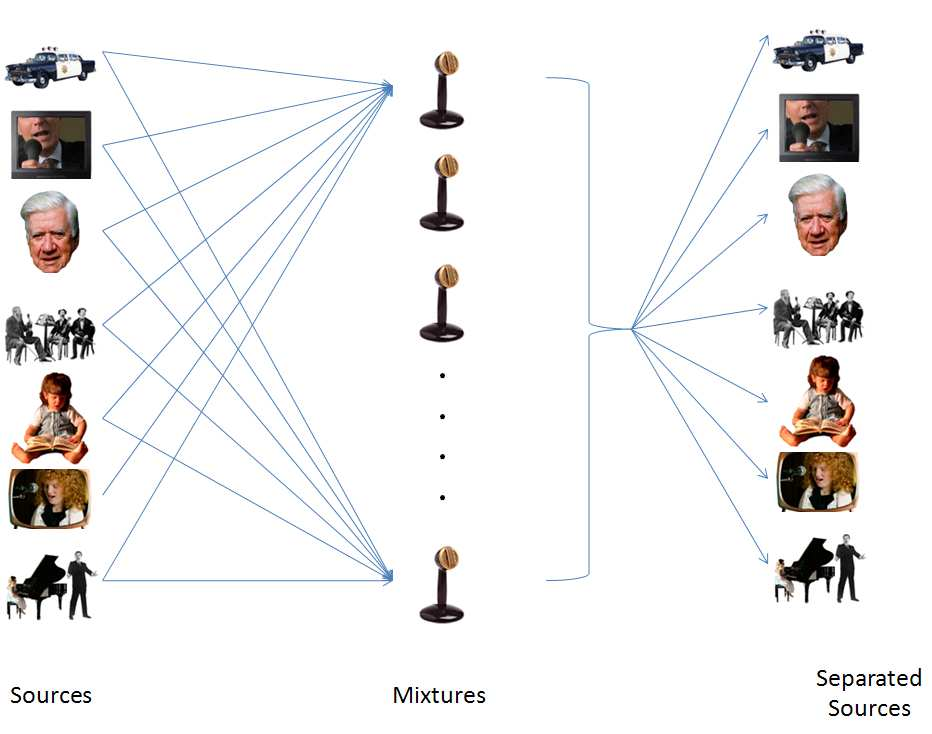
\includegraphics[width=\linewidth]{./images/bss.jpg}
  \end{subfigure}
  \caption{Blind source separation}
  \label{fig:bss}
\end{figure}

The idea behind Blind Source Separation (BSS) can be generalized to a spectrum of problems in Bioinformatics. One of the Bioinformatics problems that can be framed in BSS settings is separation of Cancer Signatures. We know that the root of any cancer is some kind of somatic mutation. There are only six distinct base substitutions (C to A, C to G, C to T, T to A, T to C, T to G) but too many cancer types. Hence it can be concluded that accumulation of these substitutions is the key difference to cause different cancers.

Analysis of the total number of each base substitution type in cancerous genoms reveals that for example in skin cancers, C to T mutations are in majority which makes sense because we know from experiment that UV causes C to T mutations. Considering the six types of base substitutions in the context of immediate previous and next base in the sequence (for example C to T mutation when previous base is A and next base is T) we would have 96 different classes of mutations. Different distributions of mutation classes are considered as cancer signatures (Figure \ref{fig:sig}).
\begin{figure}[h!]
  \centering  
  \begin{subfigure}[b]{0.5\linewidth}
    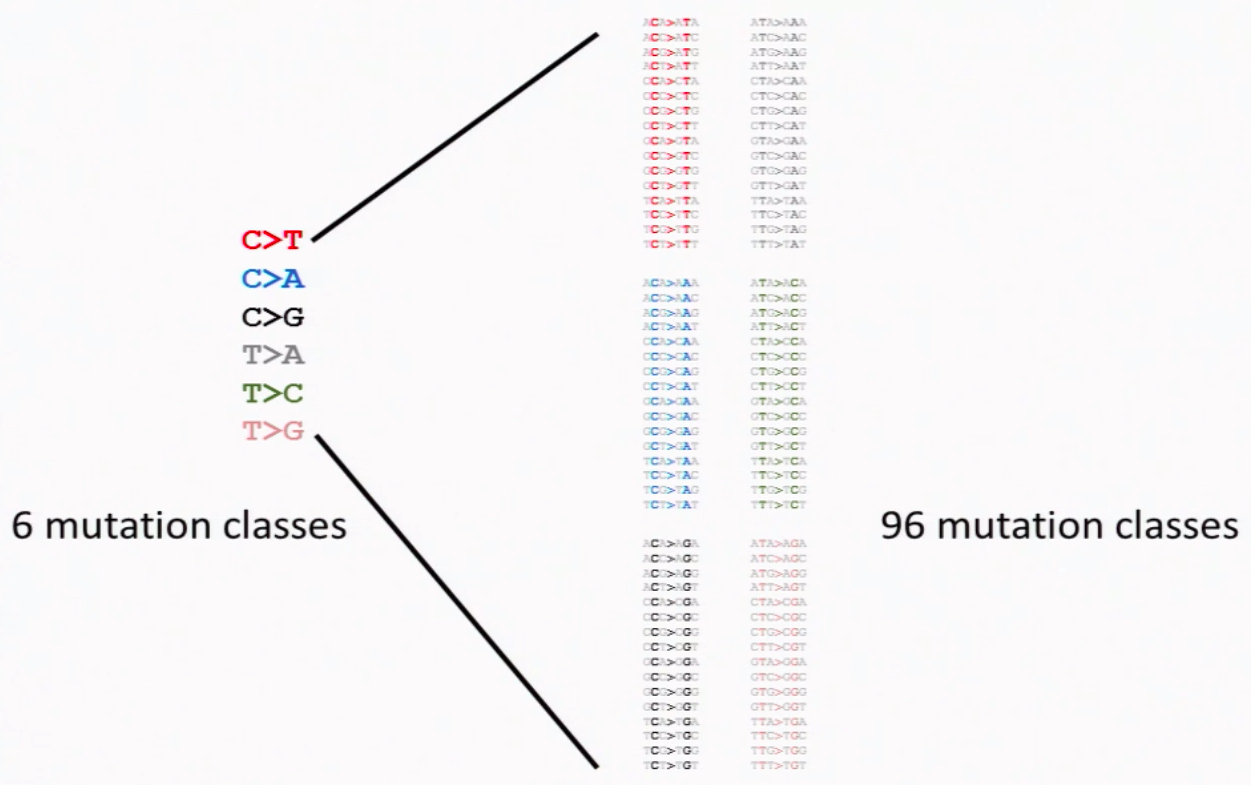
\includegraphics[width=\linewidth]{./images/sig.png}
    \caption{Mutation Classes}
  \end{subfigure}
  \begin{subfigure}[b]{0.5\linewidth}
    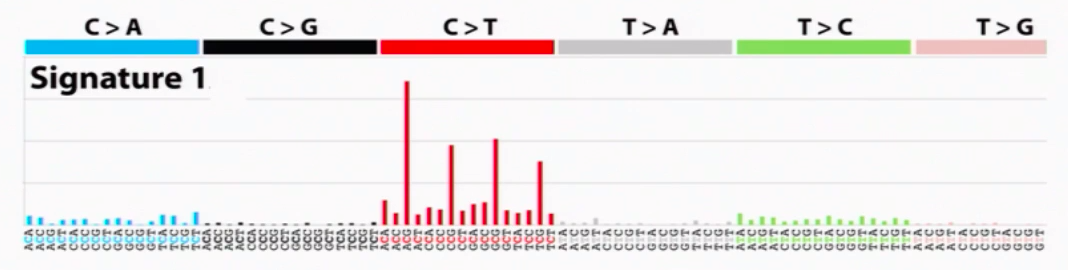
\includegraphics[width=\linewidth]{./images/sig2.png}
    \caption{A cancer signature}
  \end{subfigure}
  \caption{From Mutation clases to cancer signatures}
  \label{fig:sig}
\end{figure}

Now our challenge is to find the contribution of each cancer signature to a specific cancer type when our $input$ data is the accumulated version of base substitutions in a sequence extracted from a cancer cell.

\subsection{Reinforcement Learning}
The key idea behind Reinforcement Learning (RL) algorithms is the game of "carrot and sticks". In this context we have an agent (here our RL algorithm) taking some actions and getting rewards (and of course punishments!) from the interpreter who observes the game state consequent to taking that action from the agent. Think of a mouse (agent) in a maze (environment) trying his best (taking actions) to avoid traps (major and minor punishments) and getting to cheese (reward). In this case the designer of the game is the interpreter who either automatically or manually punishes or rewards the mouse (Figure \ref{fig:rl}).
\begin{figure}[h!]
  \centering  
  \begin{subfigure}[b]{0.7\linewidth}
    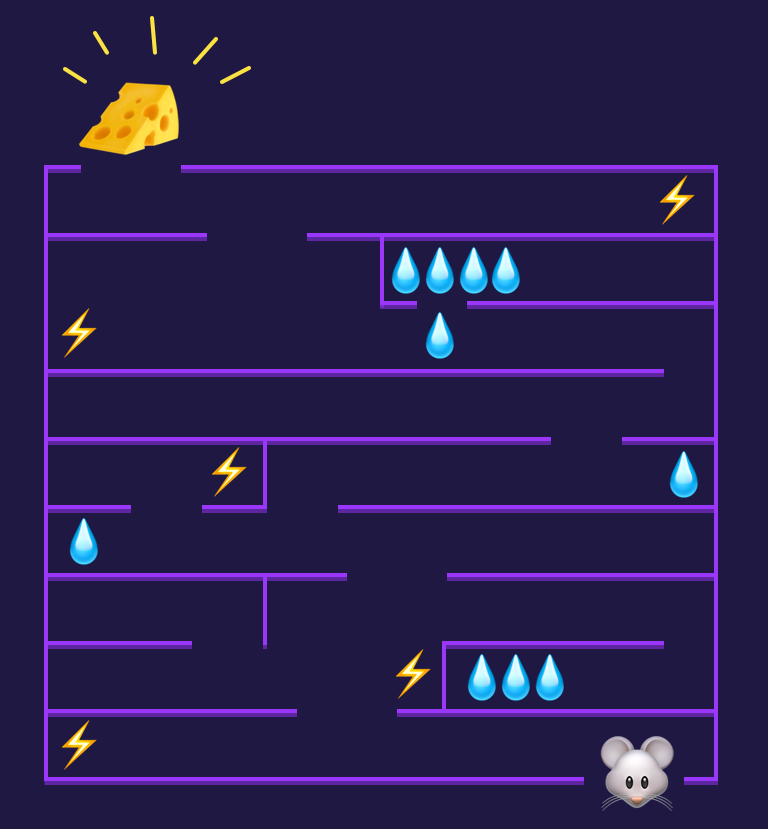
\includegraphics[width=\linewidth]{./images/rl.png}
  \end{subfigure}
  \caption{Reinforcement Learning}
  \label{fig:rl}
\end{figure}

After understanding the basics of Machine Learning it is time to roll up our sleeves and deep dive into the math behind the stuff.

\subsection{Linear regression}
Assume that we have some training data: 
$$(x[1],y[1])$$
$$(x[2],y[2])$$
$$(x[3],y[3])$$
{\centering...\par}
$$(x[n],y[n])$$
where $n$ denotes the number of our samples. We want to create a model which passes through all our data points and given a x can output its respective y. In a context where the data is 2-dimensional we can fit a simple line to our sample points:$$y=\beta_0 + \beta_1 x$$
This model consists of two parameters $\beta_0 and \beta_1$ which their value depend on our data. To find the best parameters, we have to have some notion of accuracy to evaluate our correctness (or in Machine Learning notation Falseness!). To address this problem we can define a function which takes our data and model (parameters) as input and outputs a number indicating how off we are:$$L(\beta_0,\beta_1, data) = \frac{1}{2} \sum_{i=1}^{n} y[i]-(\beta_0 + \beta_1 x[i])^2$$
Our objective is to find $\beta_0$ and $\beta_1$ so our Loss function ($L$) is at its minimum. Mathematically we can frame our objective as: 
$$\beta = \beta_0, \beta_1$$
$$ \hat{\beta_0}, \hat{\beta_1} = \argmin_\beta {L}(\beta)$$
In order to get to find best candidate for $\beta$, we can use several methods:
\begin{enumerate}
\item Gradient descent
\item Analytic method
\end{enumerate}
\subsubsection{Gradient descent}
Gradient descent is an iterative algorithm for finding best $\beta$. We start with an initial guess for $\beta$ and use the following equations to update our initial guess:
$$\beta_0 \coloneqq \beta_0 - \alpha \frac{\partial L(\beta)}{\partial \beta_0}$$
$$\beta_1 \coloneqq \beta_1 - \alpha \frac{\partial L(\beta)}{\partial \beta_1}$$
In equations above, $\alpha$ is a parameter called "Learning rate" which we will discuss later in this course. For the partial derivatives in our case we have:
$$\frac{\partial L(\beta)}{\partial \beta_0} = \frac{1}{2} \sum_{i=1}^{n} (2) (-1) (y[i]-\beta_0 + \beta_1 x[i])$$
$$\frac{\partial L(\beta)}{\partial \beta_1} = \frac{1}{2} \sum_{i=1}^{n} (2) (-x[i]) (y[i]-\beta_0 + \beta_1 x[i])$$
So the complete form of gradient descent algorithm would be:
$$\beta_0 \coloneqq \beta_0 + \alpha \sum_{i=1}^{n} (y[i]-\beta_0 + \beta_1 x[i])$$
$$\beta_1 \coloneqq \beta_1 + \alpha \sum_{i=1}^{n} (x[i]) (y[i]-\beta_0 + \beta_1 x[i])$$

This flavor of gradient descent is called "Batch". In order to update our parameters in this form, we need to go through all of our data once. This task is computation intensive and as our data grows, It would be almost impossible to compute parameters using this equations. To face this challenge we introduce another form of gradient descent called "Stochastic":
$$\beta_0 \coloneqq \beta_0 + \alpha (y[i]-\beta_0 + \beta_1 x[i])$$
$$\beta_1 \coloneqq \beta_1 + \alpha (x[i]) (y[i]-\beta_0 + \beta_1 x[i])$$

General notion of Stochastic Gradient Descent (SGD) is to update our parameters for each data point. In fact this alteration adds some noise to the minimization process but on the other hand, makes it possible to actually compute parameters using the formula (Figure \ref{fig:sgd}). 
\begin{figure}[h!]
  \centering  
  \begin{subfigure}[b]{0.5\linewidth}
    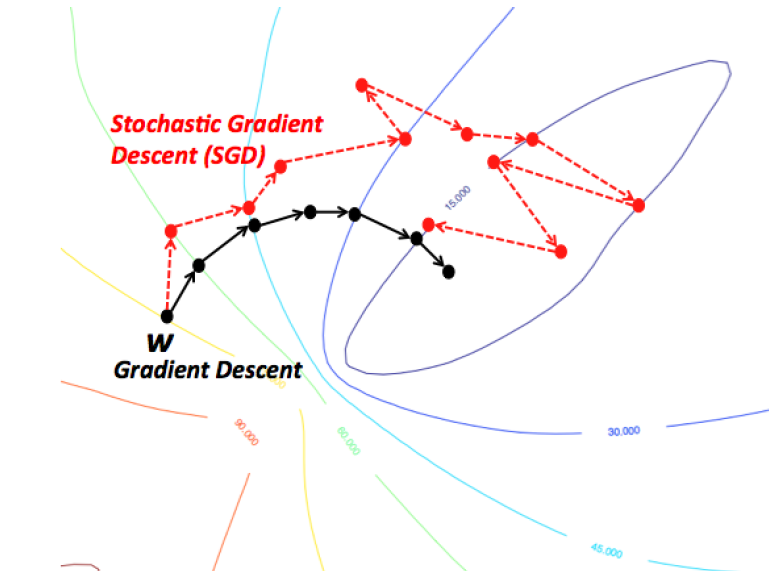
\includegraphics[width=\linewidth]{./images/sgd.png}
  \end{subfigure}
  \caption{Batch vs Stochastic Gradient Descent}
  \label{fig:sgd}
\end{figure}
\end{document}